%%%%%%%%%%%%%%%%%%%%%%
%ndss and S&P
%\documentclass[conference]{IEEEtran}
%\pagestyle{plain}

%CCS
\documentclass[sigconf, anonymous]{acmart}
\fancyhf{} % Remove fancy page headers 
\fancyhead[C]{Anonymous submission \#9999 to ACM CCS 2021} % TODO: replace 9999 with your paper number
\fancyfoot[C]{\thepage}

\setcopyright{none} % No copyright notice required for submissions
\acmConference[Anonymous Submission to ACM CCS 2021]{ACM Conference on Computer and Communications Security}{Due 15 May 2019}{London, TBD}
\acmYear{2021}
\settopmatter{printacmref=false, printccs=true, printfolios=true} % We want page numbers on submissions


%%%%%%%%%%%%%%%%%%%%%%
% \usepackage{enumitem}
\usepackage{graphicx}
\usepackage{xcolor}
\usepackage{pifont}
% \usepackage[draft]{hyperref}
\usepackage{adjustbox}
\usepackage{caption}
\usepackage{subcaption}
\usepackage{mathtools}
\usepackage{mathrsfs}
\usepackage{xspace}
\usepackage{url}
\usepackage[mode=buildnew]{standalone}
\usepackage{tikz}
\usepackage{pifont}
\usepackage{wasysym}
\usepackage{booktabs}
\usepackage{multirow}
\usetikzlibrary{positioning, trees, arrows, calc, automata}
% \usepackage{enumitem}
\usepackage{cleveref}
\usepackage{mfirstuc}
\usepackage{pifont}
%\usepackage[font={small}]{caption}
%\usepackage{enumitem}
%\usepackage[shortlabels]{enumitem}
%\usepackage{cite}
%\usepackage{flushend}
%\usepackage{hyperref}
%\usepackage{caption}

% \usepackage[
% all=normal%
% ,floats=tight%
% ,paragraphs=tight%
% % ,wordspacing=tight
% %,mathspacing=tight
% %,mathdisplays=tight
% ]{savetrees}

%\hypersetup{draft}

%% tikz figure icon definitions
% \pgfdeclareimage[width=2cm]{enclave}{icons/enclave}
% \pgfdeclareimage[width=2cm]{enclave-yellow}{icons/sgx_red}
% \pgfdeclareimage[width=2cm]{enclave-red}{icons/sgx_yellow}
% \pgfdeclareimage[width=2cm]{server}{icons/server_contoured}
% \pgfdeclareimage[width=2cm]{blockchain}{icons/blockchain}
% \pgfdeclareimage[width=2cm]{user}{icons/persons/user/user}
% \pgfdeclareimage[width=2cm]{attacker}{icons/persons/burglar}
% \pgfdeclareimage[width=1cm]{phone}{icons/smartphone}
% \pgfdeclareimage[width=2cm]{computer}{icons/devices/client}

% \pgfdeclareimage[width=2cm]{memory}{icons/computerpack/013-ram}
% \pgfdeclareimage[width=1.4cm]{gpu}{icons/computerpack/002-vga}
% \pgfdeclareimage[width=1.4cm]{mouse}{icons/computerpack/017-mouse}
% \pgfdeclareimage[width=1.4cm]{keyboard}{icons/computerpack/024-keyboard}
% \pgfdeclareimage[width=1.4cm]{screen}{icons/computerpack/018-monitor-2}
% \pgfdeclareimage[width=1.4cm]{lan}{icons/computerpack/023-lan}
% \pgfdeclareimage[width=1.4cm]{lanred}{icons/computerpack/023-lan-red}

% \definecolor{col1}{RGB}{170, 72, 59}
% \definecolor{col2}{RGB}{170,114, 59}
% \definecolor{col3}{RGB}{ 38, 93,105}
% \definecolor{col4}{RGB}{ 44,127, 66}

\definecolor{col1}{HTML}{4398D1}
\definecolor{col2}{HTML}{FF4842}
\definecolor{col3}{RGB}{ 38, 93,105}
\definecolor{col4}{RGB}{ 44,127, 66}

\definecolor{greenc}{HTML}{64c37d}
\definecolor{redc}{HTML}{e13957}

\ifstandalone
    \newcommand{\icon}[1]{../icons/#1}
\else
    \newcommand{\icon}[1]{images/icons/#1}
\fi

\newcommand{\imgmemory}{
\includegraphics[width=2.0cm]{\icon{computerpack/013-ram}}}
\newcommand{\imggpu}{
\includegraphics[width=1.4cm]{\icon{computerpack/002-vga}}}
\newcommand{\imggpusmall}{
\includegraphics[width=1.0cm]{\icon{computerpack/002-vga}}}
\newcommand{\imgmouse}{
\includegraphics[width=1.4cm]{\icon{computerpack/017-mouse}}}
\newcommand{\imgkeyboard}{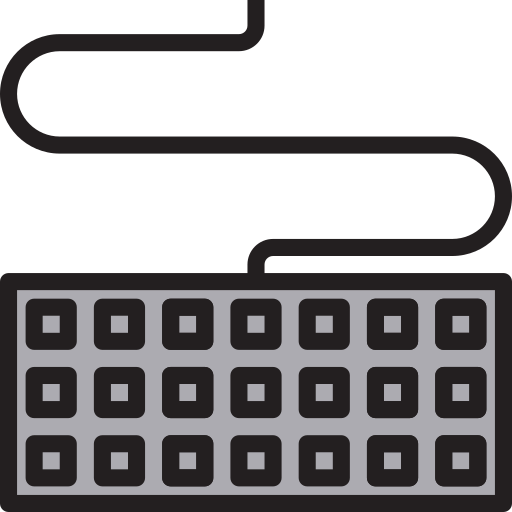
\includegraphics[width=1.4cm]{\icon{computerpack/024-keyboard}}}
\newcommand{\imgscreen}{\includegraphics[width=1.4cm]{\icon{computerpack/018-monitor}}}
\newcommand{\imglan}{
\includegraphics[width=1.4cm]{\icon{computerpack/023-lan}}}
\newcommand{\imglanred}{
\includegraphics[width=1.4cm]{\icon{computerpack/023-lan-red}}}
\newcommand{\imgcpu}{
\includegraphics[width=1.4cm]{\icon{computerpack/034-cpu}}}
\newcommand{\imgcpusmall}{
\includegraphics[width=1.0cm]{\icon{computerpack/034-cpu}}}

\newcommand{\imgdisplay}{\includegraphics[height=1.4cm]{\icon{computerpack/021-mobile}}}
\newcommand{\imgdisplaysmall}{\includegraphics[height=1.0cm]{\icon{computerpack/021-mobile}}}
\newcommand{\imgsim}{
\includegraphics[height=1.4cm]{\icon{computerpack/008-sim-card}}}
\newcommand{\imgsimsmall}{
\includegraphics[height=1.0cm]{\icon{computerpack/008-sim-card}}}
\newcommand{\imgsd}{
\includegraphics[height=1.4cm]{\icon{computerpack/011-sd-card}}}
\newcommand{\imgsdsmall}{
\includegraphics[height=1.0cm]{\icon{computerpack/011-sd-card}}}
\newcommand{\imgcamera}{\includegraphics[width=1.4cm]{\icon{computerpack/035-camera}}}
\newcommand{\imgcamerasmall}{\includegraphics[width=1.0cm]{\icon{computerpack/035-camera}}}

\newcommand{\imgenclave}{\includegraphics[width=2.0cm]{\icon{enclave}}}
\newcommand{\imgenclavesmall}{\includegraphics[width=1.4cm]{\icon{enclave}}}
\newcommand{\imgenclavesmaller}{\includegraphics[width=1.0cm]{\icon{enclave}}}
\newcommand{\imgenenclavered}{\includegraphics[width=2.0cm]{\icon{sgx_red}}}
\newcommand{\imgenenclaveredsmall}{\includegraphics[width=1.0cm]{\icon{sgx_red}}}
\newcommand{\imguser}{
\includegraphics[height=2.0cm]{\icon{persons/user/user}}}
\newcommand{\imgusersmall}{
\includegraphics[height=1.4cm]{\icon{persons/user/user}}}
\newcommand{\imgattacker}{
\includegraphics[width=2.0cm]{\icon{persons/burglar}}}
\newcommand{\imgattackersmall}{
\includegraphics[height=1.4cm]{\icon{persons/burglar}}}
\newcommand{\imgcomputer}{
\includegraphics[width=2.0cm]{\icon{devices/client}}}

\newcommand{\imglock}{\includegraphics[width=0.3cm]{\icon{lock-icon}}}
\newcommand{\imglocklarge}{\includegraphics[width=0.5cm]{\icon{lock-icon}}}
\newcommand{\imgkeyyellow}{\includegraphics[width=0.5cm]{\icon{key-yellow}}}
\newcommand{\imgkeyred}{\includegraphics[width=0.5cm]{\icon{key-red}}}
\newcommand{\imgkeyblue}{\includegraphics[width=0.5cm]{\icon{key-blue}}}
\newcommand{\imgcertred}{\includegraphics[width=0.5cm]{\icon{certificate-red}}}
\newcommand{\imgcertyellow}{\includegraphics[width=0.5cm]{\icon{certificate-yellow}}}
\newcommand{\imgcertblue}{\includegraphics[width=0.5cm]{\icon{certificate-blue}}}

\newcommand{\imgdevil}{\includegraphics[width=0.6cm]{\icon{devil}}}

\let\oldding\ding% Store old \ding in \oldding
\renewcommand{\ding}[2][1]{\scalebox{#1}{\oldding{#2}}}% Scale \oldding via optional argument

\newcommand{\zero}{\ding[1.2]{171}\xspace}
\newcommand{\one}{\ding[1.2]{172}\xspace}
\newcommand{\two}{\ding[1.2]{173}\xspace}
\newcommand{\three}{\ding[1.2]{174}\xspace}
\newcommand{\four}{\ding[1.2]{175}\xspace}
\newcommand{\five}{\ding[1.2]{176}\xspace}
\newcommand{\six}{\ding[1.2]{177}\xspace}
\newcommand{\seven}{\ding[1.2]{178}\xspace}
\newcommand{\eight}{\ding[1.2]{179}\xspace}
\newcommand{\nine}{\ding[1.2]{180}\xspace}
\newcommand{\ten}{\ding[1.2]{181}\xspace}

\newcommand{\risc}{RISC-V\xspace}
\newcommand{\ce}{controller enclave\xspace}
\newcommand{\ces}{controller enclave\xspace}
\newcommand{\Ce}{Controller enclave\xspace}
\newcommand{\Ces}{Controller enclave\xspace}
\newcommand{\app}{application enclave\xspace}
\newcommand{\App}{Application enclave\xspace}
\newcommand{\apps}{application enclaves\xspace}
\newcommand{\Apps}{Application enclaves\xspace}


\newcommand*\circled[1]{\tikz[baseline= (char.base)]{
            \node[shape=circle,draw,inner sep=0.3pt] (char) {\(#1\)};}}

\newcommand{\blue}[1]{\textcolor{black}{#1}}
\newcommand{\red}[1]{\textcolor{red}{#1}}


\newcommand{\figsaver}[0]{\vspace{-5pt}}
\newcommand{\parasaver}[0]{\vspace{-2pt}}

\newif\ifremoveall{}
\removealltrue{}

\ifremoveall{}
\newcommand{\aritra}[1]{\textbf{\emph{ #1 \colorbox{green}{[Aritra]}}}}
\newcommand{\ip}[1]{\textbf{\emph{ #1 \colorbox{cyan}{[Ivan]}}}}
\newcommand{\moritz}[1]{\textbf{\emph{ #1 \colorbox{yellow}{[Moritz]}}}}
\newcommand{\srdjan}[1]{\textbf{\emph{ #1 \colorbox{blue}{[Srdjan]}}}}
\newcommand{\todo}[1]{\textcolor{red}{TODO: \@#1}}
\newcommand{\todoref}{\textcolor{red}{[ref]}}
\newcommand{\citneed}{[\textcolor{red}{cit}] }
\else
\newcommand{\aritra}[1]{}
\newcommand{\ip}[1]{}
\newcommand{\moritz}[1]{}
\newcommand{\todo}[1]{}
\newcommand{\todoref}[1]{}
\newcommand{\citneed}[1]{}
\fi


\newcommand{\name}{\textsc{PIE}\xspace}
\newcommand{\tool}{\textsc{\name{} API}\xspace}
\newcommand{\device}{\textsc{Device}\xspace}

\newcommand{\usb}{\texttt{USB}\xspace}
\newcommand{\tls}{\texttt{TLS}\xspace}

\def\nameenclave{platform-wide enclave\xspace}
\def\Nameenclave{Platform-wide enclave\xspace}

\newcommand{\sphw}[0]{specialized hardware\xspace}
\newcommand{\Sphw}[0]{Specialized hardware\xspace}


%%%%%%%%%%%%%%%%%%%%%%
%savetrees
\usepackage[
all=normal,floats=tight
,paragraphs=tight
% ,wordspacing=tight
,mathspacing=tight
% ,mathdisplays=tight
]{savetrees}
%%%%%%%%%%%%%%%%%%%%%%

% \newcommand{\myparagraph}[1]{\par\emph{#1.}\xspace}
\newcommand{\myparagraph}[1]{\paragraph{#1}}

\newcounter{para}
% \newcommand{\mypara}[1]{\refstepcounter{para}\emph{\thepara}.\space\emph{#1}.\xspace}
\newcommand{\mypara}[1]{\refstepcounter{para}\paragraph{\thepara.\space{}#1}}
% \newcommand{\mypara}[1]{\paragraph{#1}}
%\newcommand\mypara{\par\refstepcounter{para}\thepara\space}

%------------------------------------------------------------------------------
%                                Space savers.
%------------------------------------------------------------------------------
% This mylist environment indents items, and saves less space than the above.
\newcounter{myctr}
\newenvironment{mylist}{\begin{list}{\arabic{myctr}.}
{\usecounter{myctr}
\setlength{\topsep}{1mm}\setlength{\itemsep}{0.5mm}
\setlength{\parsep}{0.5mm}
\setlength{\itemindent}{1mm}\setlength{\partopsep}{0mm}
\setlength{\labelwidth}{-2mm}
\setlength{\leftmargin}{0mm}}}{\end{list}}

\newenvironment{mylist_indent}{\begin{list}{\arabic{myctr}.}
{\usecounter{myctr}
\setlength{\topsep}{1mm}\setlength{\itemsep}{0.5mm}
\setlength{\parsep}{0.5mm}
\setlength{\itemindent}{1.5mm}\setlength{\partopsep}{1mm}
\setlength{\labelwidth}{-2mm}
\setlength{\leftmargin}{1mm}}}{\end{list}}

% Space saving List environment for itemizing.
\newenvironment{mybullet}{\begin{list}{\bullet}
{\setlength{\topsep}{1mm}\setlength{\itemsep}{0.5mm}
\setlength{\parsep}{0.5mm}
\setlength{\itemindent}{0mm}\setlength{\partopsep}{0mm}
\setlength{\labelwidth}{-2mm}
\setlength{\leftmargin}{0mm}}}{\end{list}}


% Break characters in the reference
\expandafter\def\expandafter\UrlBreaks\expandafter{\UrlBreaks
  \do\a\do\b\do\c\do\d\do\e\do\f\do\g\do\h\do\i\do\j
  \do\k\do\l\do\m\do\n\do\o\do\p\do\q\do\r\do\s\do\t
  \do\u\do\v\do\w\do\x\do\y\do\z\do\A\do\B\do\C\do\D
  \do\E\do\F\do\G\do\H\do\I\do\J\do\K\do\L\do\M\do\N
  \do\O\do\P\do\Q\do\R\do\S\do\T\do\U\do\V\do\W\do\X
  \do\Y\do\Z}
  
  